\chapter{Design}


\section{Document Database}
For the document database, we will use MongoDB. MongoDB is a NoSQL database that stores data in flexible, JSON-like documents. It is a popular choice for applications that require flexibility and scalability. MongoDB is a document database, which means it stores data in JSON-like documents. These documents are flexible, meaning they can have different fields and structures. This makes MongoDB a good choice for applications that require flexibility in their data model. MongoDB is also a scalable database, meaning it can handle large amounts of data and traffic. It is designed to scale out, meaning you can add more servers to handle more traffic. This makes MongoDB a good choice for applications that need to scale quickly.
\newline
\newline
\textbf{Collections}
The database will have the following collections:
\begin{itemize}
    \item Anime: This collection will store information about anime, such as titles, tags, and synopsis.
    \item Manga: This collection will store information about manga, such as titles, genres, and authors.
    \item Reviews: This collection will store user ratings and comments for media content.
    \item Users: This collection will store user data, such as usernames, passwords, email addresses, gender and location.

\end{itemize}
\newpage
\textbf{MongoDB document example}
\newline
Anime:
\begin{mdframed}[backgroundcolor=yellow!20, innerleftmargin=10pt, innerrightmargin=10pt]
    \begin{lstlisting}[language=java]
{
  "_id": "65789bb52f5d29465d0abcfb",
  "title": "0",
  "type": "SPECIAL",
  "episodes": 1,
  "status": "FINISHED",
  "picture": "https://cdn.myanimelist.net/images/anime/12/81160.jpg",
  "tags": [
    "drama",
    "female protagonist",
    "indefinite",
    "music",
    "present"
  ],
  "producers": "Sony Music Entertainment",
  "studios": "Minakata Laboratory",
  "synopsis": "This music video tells how a shy girl with a secret love and curiosity...",
  "latest_reviews": [
    {
      "id": "657b301306c134f18884924c",
      "date": "2023-10-03T22:00:00.000+00:00",
      "rating": 4,
      "user": {
        "id": "6577877ce68376234760745c",
        "username": "Tolstij_Trofim",
        "picture": "https://thypix.com/wp-content/uploads/2021/10/manga-profile-picture-10..."
      }
    },
  ],
  "anime_season": {
    "season": "FALL",
    "year": 2013
  },
  "average_rating": 6.7,
  "avg_rating_last_update": true,
  "likes": 4
}
    \end{lstlisting}
\end{mdframed}

\newpage
Manga:
\begin{mdframed}[backgroundcolor=yellow!20, innerleftmargin=10pt, innerrightmargin=10pt]
    \begin{lstlisting}[language=java]
{
  "_id": "657ac61bb34f5514b91ea223",
  "title": "Berserk",
  "type": "MANGA",
  "status": "ONGOING",
  "genres": [
    "Action",
    "Adventure",
    "Award Winning",
    "Drama",
    "Fantasy",
    "Horror",
    "Supernatural"
  ],
  "themes": [
    "Gore",
    "Military",
    "Mythology",
    "Psychological"
  ],
  "demographics": [
    "SEINEN"
  ],
  "authors": [
    {
      "id": 1868,
      "role": "Story & Art",
      "name": "Kentarou Miura"
    },
    {
      "serializations": "Young Animal"
    }
  ],
  "synopsis": "Guts, a former mercenary now known as the \"Black Swordsman,\" is out fo...",
  "title_english": "Berserk",
  "start_date": "1989-08-25T00:00:00.000+00:00",
  "picture": "https://cdn.myanimelist.net/images/manga/1/157897l.jpg",
  "average_rating": 3.33,
  "latest_reviews": [
    {
      "user": {
        "id": "6577877be683762347605ce7",
        "username": "calamity_razes",
        "picture": "https://imgbox.com/7MaTkBQR"
      },
      "date": "2012-12-15T00:00:00.000+00:00",
      "comment": "An insult to the art of manga; avoid at all costs.",
      "id": "657b302206c134f18886f5ef"
    },
  ],
  "anime_season": {
    "season": "FALL",
    "year": 2013
  },
  "average_rating": 6.7,
  "avg_rating_last_update": true,
  "likes": 4
}
    \end{lstlisting}
\end{mdframed}
\newpage
Reviews:
\begin{mdframed}[backgroundcolor=yellow!20, innerleftmargin=10pt, innerrightmargin=10pt]
    \begin{lstlisting}[language=java]
{
  "_id": "657b300806c134f18882f2f1",
  "user": {
    "id": "6577877be68376234760596d",
    "username": "Dragon_Empress",
    "picture": "images/account-icon.png",
    "location": "Columbus, Georgia",
    "birthday": "1987-07-29T00:00:00.000+00:00",
    "rating": 7
  },
  "anime": {
    "id": "65789bbc2f5d29465d0b18b7",
    "title": "Slayers Revolution",
    "date": "2023-07-23T06:27:54.000+00:00",
    "comment": "Above-average quality in animation and soundtrack."
  }
}
    \end{lstlisting}
\end{mdframed}

Users:
\begin{mdframed}[backgroundcolor=yellow!20, innerleftmargin=10pt, innerrightmargin=10pt]
    \begin{lstlisting}[language=java]
{
  "_id": "6577877be683762347605859",
  "email": "xdavis@example.com",
  "password": "290cb38a679d5eb68d11b9ea1e21f48234eba6de19f95612dbcb70ce0c7e4e78",
  "description": "Liberating the mind from stress with the power of anime zen.",
  "picture": "https://thypix.com/wp-content/uploads/2021/10/manga-profile-picture-44",
  "username": "Xinil",
  "gender": "Male",
  "birthday": "1985-03-04T00:00:00.000+00:00",
  "location": "Libya",
  "joined_on": "2014-05-29T00:00:00.000+00:00",
  "app_rating": 5,
  "followed": 40,
  "followers": 29
}
    \end{lstlisting}
\end{mdframed}

\textbf{Indexes}
\newline
We created two indexes in the reviews collection to improve query performance. One for the users id and another for the anime and manga id. This will allow us to quickly retrieve reviews for a specific user or media content. 

\section{Graph Database}
For the graph database, we will use Neo4j. Neo4j is a graph database that stores data in nodes and relationships. It is a popular choice for applications that require complex relationships between data. Neo4j is a graph database, which means it stores data in nodes and relationships. Nodes represent entities, such as users or products, and relationships represent connections between nodes. This makes Neo4j a good choice for applications that require complex relationships between data. Neo4j is also a scalable database, meaning it can handle large amounts of data and traffic. It is designed to scale out, meaning you can add more servers to handle more traffic. This makes Neo4j a good choice for applications that need to scale quickly.



\textbf{Nodes}



The database will have the following nodes:
\begin{itemize}
    \item User: This node will store information about users, such as id, usernames, and picture.
    \item Anime: This node will store information about anime, such as id, titles and picture.
    \item Manga: This node will store information about manga, such as id, titles and picture.
\end{itemize}

\textbf{Relationships}


The database will have the following relationships:
\begin{itemize}
    \item LIKE: This relationship will connect users to anime and manga nodes. It will store the date when the user liked the media content.
    \item FOLLOW: This relationship will connect users to other users. 
\end{itemize}

\begin{figure}[htbp]
    \centering
    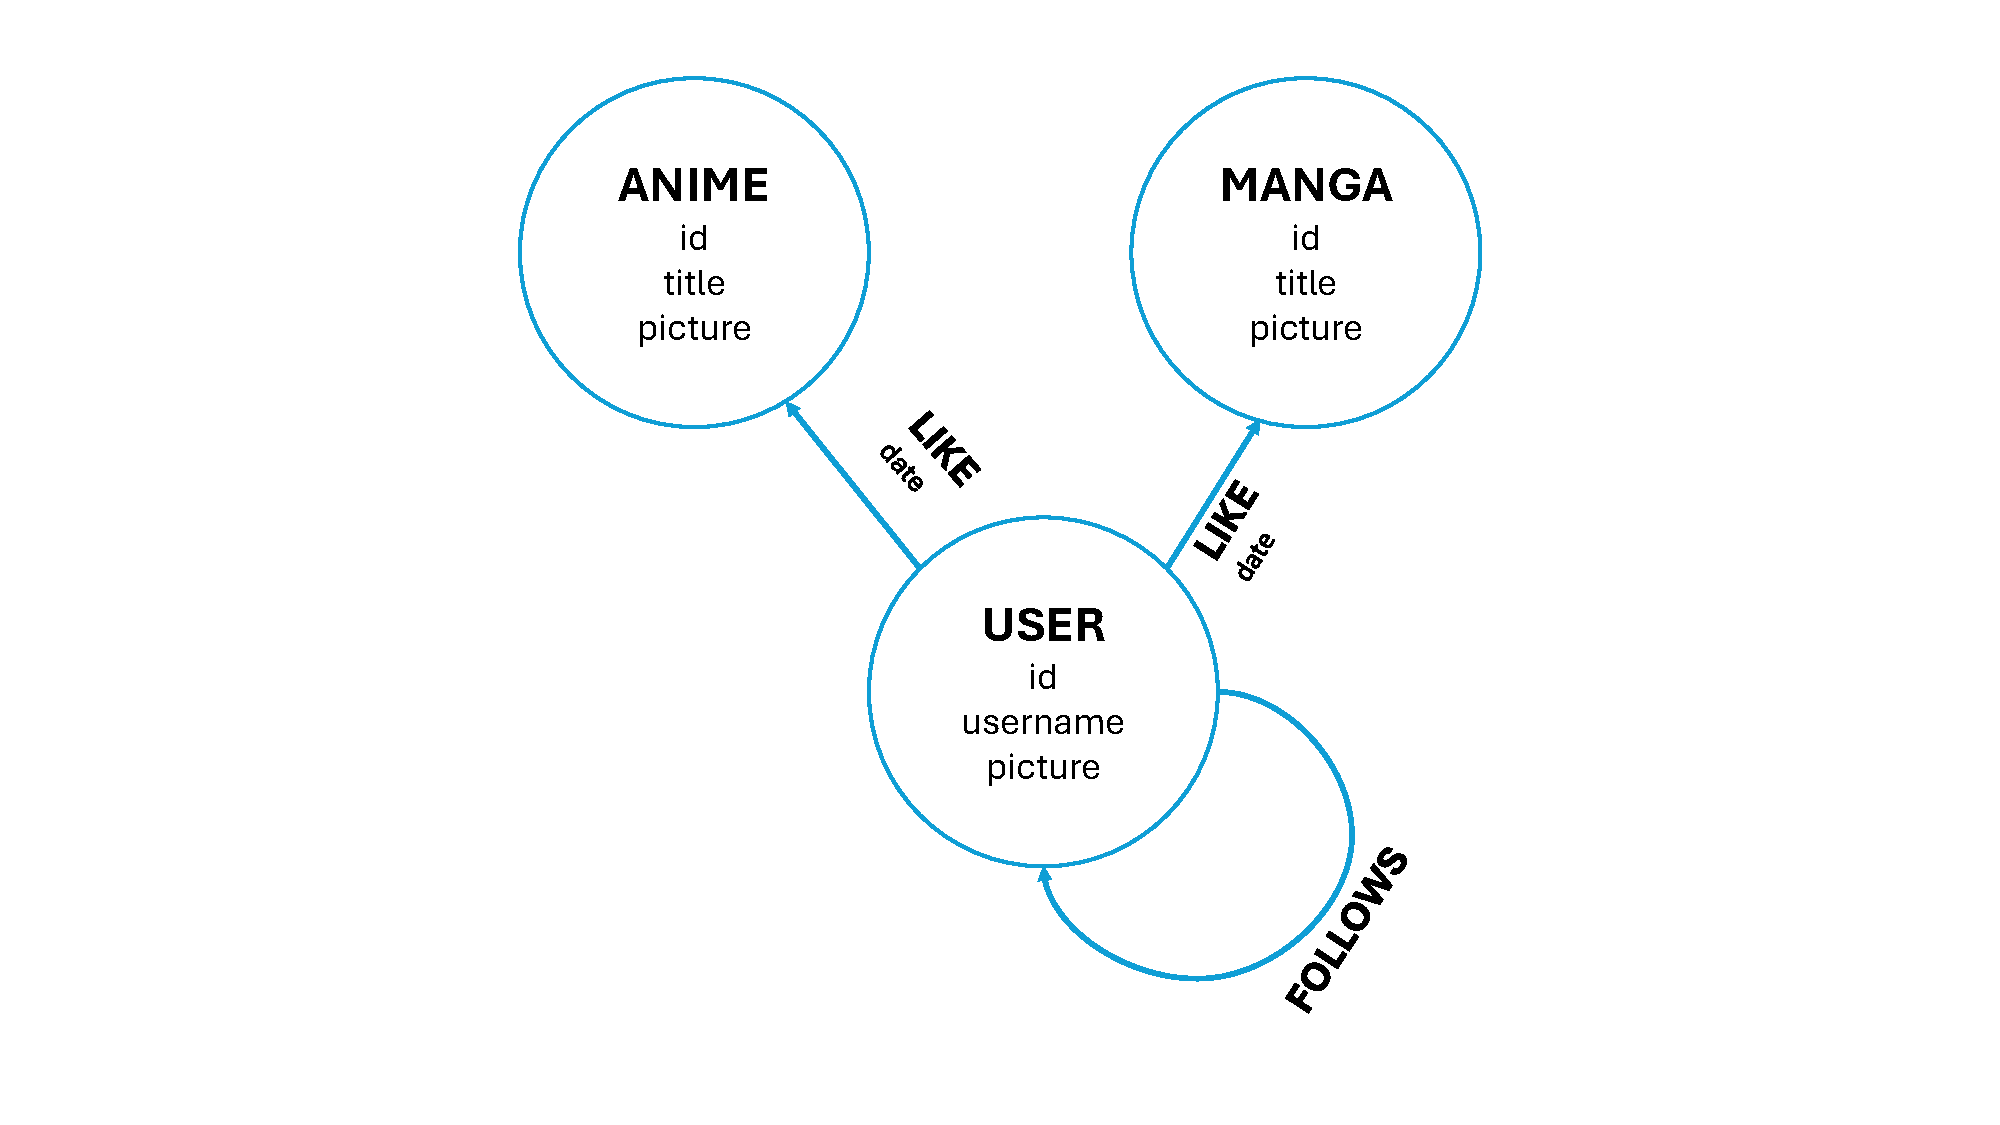
\includegraphics[width=\textwidth]{Media/graph.pdf}
    \caption{GraphDB}
    \label{fig:GraohDB}
\end{figure}
